% ==============================================================================
\chapter{Reduced Order Modeling (ROM) \& Hyper-Reduction}
\label{ch:rom}
% ==============================================================================

To bypass the severe computational overhead of the Full Order Model (FOM) simulations, we implement a projection-based Reduced Order Modeling (ROM) framework. This chapter details the progression of the model reduction strategies, culminating in the client-side Digital Twin implementation.

\section{The Full-Order Bottleneck and Model Reduction Strategy}
\subsection{Why Reduced Order Modeling? (Motivation)}
The high-fidelity Full Order Model (FOM) developed in Chapter \ref{ch:fom} provides precise dynamic responses by solving the discretized NURBS-based equations of motion. However, this accuracy comes at a massive computational cost. A single time-step requires assembling the parameterized global matrices in its full physical dimension ($N = 6,564$ degrees of freedom) and solving the linear system. 

When structural properties or geometric shapes change dynamically (such as notch updates mid-simulation), the global stiffness matrix must be re-assembled online, which scales with the mesh size $\mathcal{O}(N)$. Solving this high-dimensional system at each time step prevents real-time interactivity. To deploy this simulation in an interactive client-side web application (a Digital Twin), we must bypass this full-order bottleneck. Reduced Order Modeling (ROM) solves this by projecting the governing equations onto a low-dimensional coordinate space, replacing the expensive full-mesh calculations with lightweight, generalized coordinate solves.

\subsection{What Do We Need to Achieve? (Reduction Targets)}
To construct a successful and reliable reduced-order representation of the structural continuum, the ROM must satisfy the following critical requirements:
\begin{enumerate}
    \item \textbf{Low Computational Time}: The online solve and assembly time per step must be under a few milliseconds (ideally $<1.5\text{ ms}$) to fit comfortably within the rendering and interaction budget ($20$--$60$ FPS) of standard web browsers.
    \item \textbf{Low Approximation Error (High Fidelity)}: The reduced model must maintain high physical accuracy (relative $L_2$ displacement error $< 0.1\%$) and capture stress concentration behaviors near the notches exactly.
    \item \textbf{Geometric and Parametric Compatibility}: The reduced basis must accommodate dynamic shape modifications (varying notch positions $x_c$ and radii $r$) without suffering from vector space incompatibility or requiring expensive online re-training.
    \item \textbf{Spectral Conservation}: The projection must preserve the fundamental dynamic properties of the structure, such as conserving natural frequencies and mode shapes with minimal eigenvalue drift.
\end{enumerate}

\subsection{The Model Reduction Recipe}
To achieve these targets, we formulate a projection-based reduction methodology divided into offline (computationally intensive, executed once) and online (lightweight, executed in real-time) stages. The step-by-step recipe is:

\begin{tcolorbox}[colback=blue!5!white,colframe=blue!65!black,title={\textbf{Step 1: Pullback Mapping to a Static Reference Domain}}, fonttitle=\bfseries]
To handle shape parameterization (changing geometry), we pull back the governing equations from the parameter-dependent physical domain $\Omega(\boldsymbol{\mu})$ to a fixed reference configuration $\hat{\Omega}$. This ensures that all snapshot vectors and bases reside in the same vector space, enabling consistent projections.
\end{tcolorbox}

\begin{tcolorbox}[colback=blue!5!white,colframe=blue!65!black,title={\textbf{Step 2: Offline Snapshot Collection (Data Generation)}}, fonttitle=\bfseries]
Run high-fidelity FOM simulations across representative combinations of geometric and physical parameters $\boldsymbol{\mu} \in \mathcal{D}$ (e.g., notch positions and radii under typical loading paths). The resulting displacement fields are compiled into a snapshot matrix $\mathbf{S}_u$.
\end{tcolorbox}

\begin{tcolorbox}[colback=blue!5!white,colframe=blue!65!black,title={\textbf{Step 3: Proper Orthogonal Decomposition (Basis Construction)}}, fonttitle=\bfseries]
Perform a Singular Value Decomposition (SVD) on the snapshot matrix $\mathbf{S}_u$. The left singular vectors corresponding to the largest singular values represent the dominant modes of deformation, forming the reduced basis matrix $\boldsymbol{\Phi} \in \mathbb{R}^{N \times r}$.
\end{tcolorbox}

\begin{tcolorbox}[colback=blue!5!white,colframe=blue!65!black,title={\textbf{Step 4: Hyper-Reduction Training (ECSW NNLS Optimization)}}, fonttitle=\bfseries]
To break the online assembly bottleneck (where matrix assembly still scales with the full mesh size $E$), we train the Energy-Conserving Sampling and Weighting (ECSW) hyper-reduction method. By solving a Non-Negative Least Squares (NNLS) optimization, we select a sparse subset of active elements $E^* \subset E$ and positive integration weights $w_e$ that approximate the internal forces.
\end{tcolorbox}

\begin{tcolorbox}[colback=blue!5!white,colframe=blue!65!black,title={\textbf{Step 5: Online Real-Time Simulation and State Projection}}, fonttitle=\bfseries]
During the interactive session, the web browser solver executes the reduced integration loops exclusively over the sparse subset of active elements $E^*$. When the user modifies shape parameters mid-simulation, the solver projects the current physical states onto the new parametric basis (transient state projection) to maintain physical continuity, solves the $r \times r$ system, and reconstructs the full physical field for real-time visualization.
\end{tcolorbox}


This chapter details the mathematical formulation and numerical verification of this workflow: Section \ref{sec:galerkin_rom} formulates the standard Galerkin ROM; Section \ref{sec:pullback} presents the reference configuration mapping; Section \ref{sec:state_projection} addresses parameter updates and state projection; Section \ref{sec:ecsw} details the hyper-reduction framework; Section \ref{sec:mvc} details the client-side web implementation; and Section \ref{sec:benchmarks} evaluates the performance.



\section{Standard Galerkin ROM (Dimensionality Reduction)} \label{sec:galerkin_rom}
In Section 5.1, the high-fidelity spatial displacement vector $\vect{U}(t) \in \mathbb{R}^N$ is projected onto a low-dimensional subspace spanned by a Reduced Basis matrix $\boldsymbol{\Phi} \in \mathbb{R}^{N \times r}$ ($r \ll N$):
\begin{equation}
    \vect{U}(t) \approx \boldsymbol{\Phi} \vect{q}(t)
\end{equation}
where $\vect{q}(t) \in \mathbb{R}^r$ represents the vector of reduced coordinates (amplitudes). The reduced basis matrix $\boldsymbol{\Phi}$ is constructed via Proper Orthogonal Decomposition (POD) from snapshots of the FOM displacement field. 

To determine the number of modes $r$ needed to represent the displacement field accurately, we evaluate the cumulative modal energy fraction $\eta(r)$ and the corresponding relative $L_2$ projection error $\epsilon(r)$, defined as:
\begin{equation}
    \eta(r) = \frac{\sum_{i=1}^{r} \sigma_i^2}{\sum_{j=1}^{d} \sigma_j^2}, \quad \epsilon(r) = \sqrt{1 - \eta(r)}
\end{equation}
where $\sigma_i$ represents the $i$-th singular value obtained from the Singular Value Decomposition (SVD) of the snapshot matrix $\mathbf{S}_u$, and $d$ is the total number of snapshots. In this work, a singular value energy ratio threshold of $\eta(r) \ge 99.99\%$ (corresponding to a relative projection error $\epsilon(r) \le 0.01\%$) is enforced to truncate the basis dimension to $r$, guaranteeing that all dominant deformation dynamics are captured while filtering numerical noise. The convergence of the relative $L_2$ reconstruction error as a function of the number of POD modes is shown in Figure \ref{fig:pod_energy_decay}.

\begin{figure}[htbp]
    \centering
    \begin{subfigure}{0.46\textwidth}
        \centering
        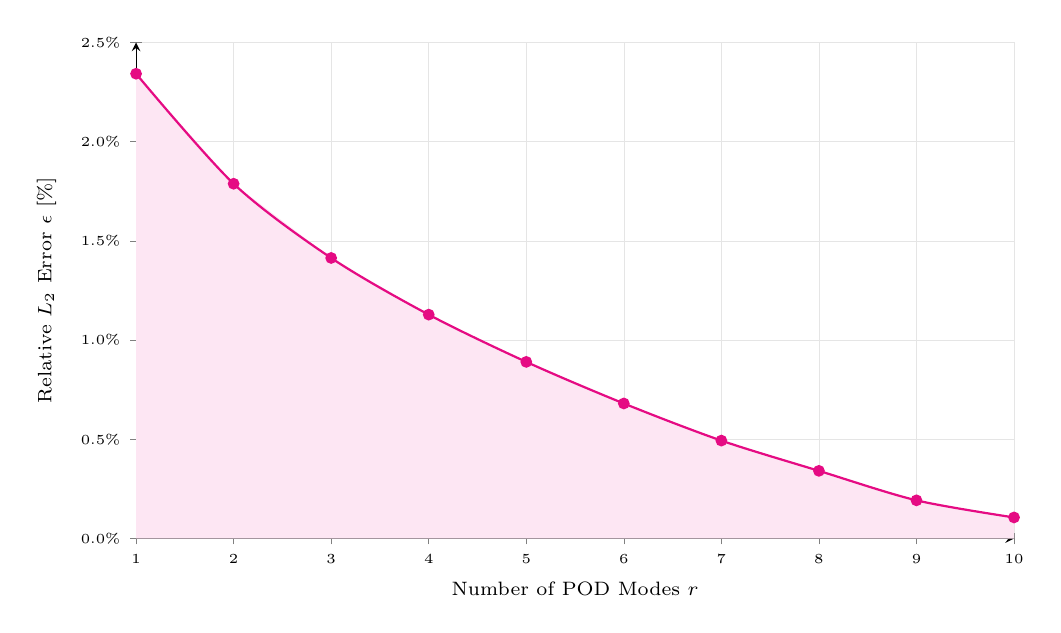
\begin{tikzpicture}
            \begin{axis}[
                width=1.05\textwidth,
                height=0.65\textwidth,
                xlabel={Number of POD Modes $r$},
                ylabel={Relative $L_2$ Error $\epsilon$ [\%]},
                xmin=1, xmax=10,
                ymin=0, ymax=2.5,
                xtick={1,2,3,4,5,6,7,8,9,10},
                ytick={0, 0.5, 1.0, 1.5, 2.0, 2.5},
                yticklabels={0.0\%, 0.5\%, 1.0\%, 1.5\%, 2.0\%, 2.5\%},
                grid=both,
                grid style={line width=.1pt, draw=gray!10},
                major grid style={line width=.2pt, draw=gray!20},
                axis lines=left,
                enlargelimits=false,
                x tick label style={font=\tiny},
                y tick label style={font=\tiny},
                xlabel style={font=\scriptsize},
                ylabel style={font=\scriptsize, yshift=0.2em},
            ]
                \addplot[
                    fill=magenta!10,
                    draw=none,
                ] coordinates {
                    (1, 2.3424)
                    (2, 1.7880)
                    (3, 1.4139)
                    (4, 1.1283)
                    (5, 0.8902)
                    (6, 0.6806)
                    (7, 0.4935)
                    (8, 0.3410)
                    (9, 0.1924)
                    (10, 0.1062)
                } \closedcycle;

                \addplot[
                    color=magenta!85!purple,
                    mark=*,
                    thick,
                    smooth,
                    mark options={fill=magenta!85!purple, draw=magenta!85!purple, line width=1pt, scale=0.8}
                ] coordinates {
                    (1, 2.3424)
                    (2, 1.7880)
                    (3, 1.4139)
                    (4, 1.1283)
                    (5, 0.8902)
                    (6, 0.6806)
                    (7, 0.4935)
                    (8, 0.3410)
                    (9, 0.1924)
                    (10, 0.1062)
                };
            \end{axis}
        \end{tikzpicture}
        \caption{Relative $L_2$ projection error $\epsilon(r)$.}
        \label{fig:pod_error}
    \end{subfigure}
    \hfill
    \begin{subfigure}{0.46\textwidth}
        \centering
        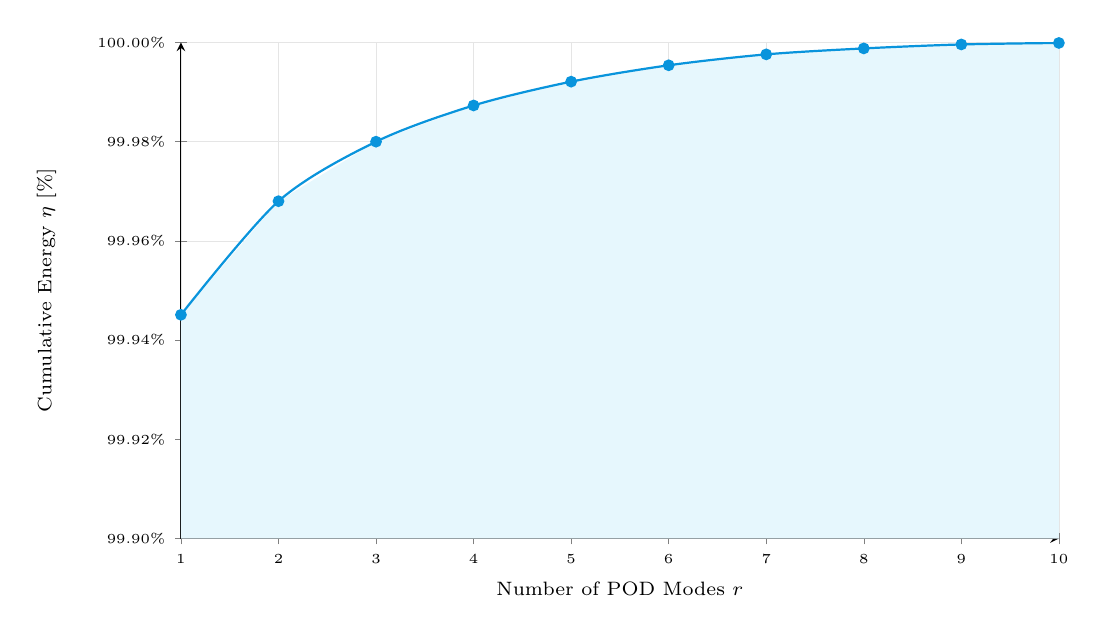
\begin{tikzpicture}
            \begin{axis}[
                width=1.05\textwidth,
                height=0.65\textwidth,
                xlabel={Number of POD Modes $r$},
                ylabel={Cumulative Energy $\eta$ [\%]},
                xmin=1, xmax=10,
                ymin=99.9, ymax=100.0,
                xtick={1,2,3,4,5,6,7,8,9,10},
                ytick={99.9, 99.92, 99.94, 99.96, 99.98, 100.0},
                yticklabels={99.90\%, 99.92\%, 99.94\%, 99.96\%, 99.98\%, 100.00\%},
                grid=both,
                grid style={line width=.1pt, draw=gray!10},
                major grid style={line width=.2pt, draw=gray!20},
                axis lines=left,
                enlargelimits=false,
                x tick label style={font=\tiny},
                y tick label style={font=\tiny},
                xlabel style={font=\scriptsize},
                ylabel style={font=\scriptsize, yshift=0.8em},
            ]
                \addplot[
                    fill=cyan!10,
                    draw=none,
                ] coordinates {
                    (1, 99.9451)
                    (2, 99.9680)
                    (3, 99.9800)
                    (4, 99.9873)
                    (5, 99.9921)
                    (6, 99.9954)
                    (7, 99.9976)
                    (8, 99.9988)
                    (9, 99.9996)
                    (10, 99.9999)
                } \closedcycle;

                \addplot[
                    color=cyan!80!blue,
                    mark=*,
                    thick,
                    smooth,
                    mark options={fill=cyan!80!blue, draw=cyan!80!blue, line width=1pt, scale=0.8}
                ] coordinates {
                    (1, 99.9451)
                    (2, 99.9680)
                    (3, 99.9800)
                    (4, 99.9873)
                    (5, 99.9921)
                    (6, 99.9954)
                    (7, 99.9976)
                    (8, 99.9988)
                    (9, 99.9996)
                    (10, 99.9999)
                };
            \end{axis}
        \end{tikzpicture}
        \caption{Cumulative modal energy fraction $\eta(r)$.}
        \label{fig:pod_energy}
    \end{subfigure}
    \caption{Proper Orthogonal Decomposition (POD) spectral convergence analysis showing both (a) relative projection error decay and (b) cumulative energy fraction as a function of the reduced basis size $r$.}
    \label{fig:pod_energy_decay}
\end{figure}

Applying the Galerkin projection to the linear semi-discrete equation of motion yields the projected governing system of dimension $r$:
\begin{equation}
    \mathbf{M}_{r} \ddot{\vect{q}}(t) + \mathbf{C}_{r} \dot{\vect{q}}(t) + \mathbf{K}_{r}(\boldsymbol{\mu}) \vect{q}(t) = \mathbf{F}_{r}(t)
\end{equation}
where the reduced mass, stiffness, and damping matrices, and the projected force vector are defined as:
\begin{equation}
    \mathbf{M}_{r} = \boldsymbol{\Phi}^T \hat{\mathbf{M}} \boldsymbol{\Phi}, \quad \mathbf{K}_{r}(\boldsymbol{\mu}) = \boldsymbol{\Phi}^T \hat{\mathbf{K}}(\boldsymbol{\mu}) \boldsymbol{\Phi}, \quad \mathbf{C}_{r} = \boldsymbol{\Phi}^T \hat{\mathbf{C}} \boldsymbol{\Phi}, \quad \mathbf{F}_{r}(t) = \boldsymbol{\Phi}^T \hat{\mathbf{F}}_{\text{ext}}(t)
\end{equation}

For very low-dimensional systems (e.g., $r = 2$), the effective system of equations $\mat{K}_{\text{eff},r}\Delta \vect{q} = \vect{R}_r$ is solved analytically at each time step using \textbf{Cramer's Rule}:
\begin{equation}
    \Delta q_1 = \frac{R_1 K_{22} - R_2 K_{12}}{\det(\mathbf{K}_{\text{eff}, r})}, \quad \Delta q_2 = \frac{K_{11} R_2 - K_{21} R_1}{\det(\mathbf{K}_{\text{eff}, r})}
\end{equation}
which bypasses the expensive global Gaussian elimination solves.

Despite this, the standard Galerkin ROM suffers from the \textbf{assembly bottleneck}: when the shape parameter $\boldsymbol{\mu}$ changes, the global stiffness matrix $\hat{\mathbf{K}}(\boldsymbol{\mu})$ must still be assembled in its full physical dimension $N$ before projecting it to $\mathbf{K}_r(\boldsymbol{\mu})$. Thus, the online computational cost still scales with the size of the full mesh $\mathcal{O}(N)$, preventing real-time evaluation.


% ==============================================================================
\section{Reference Configuration Mapping} \label{sec:pullback}
% ==============================================================================
Constructing a shape-parametric ROM capable of real-time predictions under varying geometric parameters $\boldsymbol{\mu} \in \mathcal{D}$ requires a mathematically rigorous representation of the parameterized equations. 

\subsection{Physical-Domain FOM (The Classical Remeshing Approach)}
In a classical physical-domain formulation, the Full Order Model (FOM) equations of motion are resolved directly on the physical parameter-dependent domain $\Omega(\boldsymbol{\mu})$:
\begin{equation}
\mat{M}(\boldsymbol{\mu})\ddot{\vect{U}}(t) + \mat{C}(\boldsymbol{\mu})\dot{\vect{U}}(t) + \mathbf{F}_{\text{int}}(\vect{U}(t); \boldsymbol{\mu}) = \mathbf{F}_{\text{ext}}(t)
\end{equation}
This approach presents severe limitations:
\begin{enumerate}
    \item \textbf{Vector Space Incompatibility}: SVD-based basis extraction (POD) requires snapshot vectors to lie in the same vector space. If the mesh is regenerated for each parameter set, the dimensions $N(\boldsymbol{\mu})$ and nodal locations vary, preventing SVD analysis without complex interpolations.
    \item \textbf{High Assembly Cost}: Remeshing and re-assembling the stiffness and mass matrices over varying physical domains introduces massive online computational overhead.
    \item \textbf{Loss of Parametric Differentiability}: Discrete mesh regeneration introduces numerical noise, destroying the smooth parameter-to-solution mapping required for sensitivity analysis.
\end{enumerate}

\subsection{FOM Pullback to a Static Reference Configuration}
To resolve these issues, the governing equations are pulled back from the parameterized physical domain $\Omega(\boldsymbol{\mu})$ to a fixed reference configuration $\hat{\Omega}$ using the smooth, parameterized geometric mapping:
\begin{equation}
\vect{x} = \boldsymbol{\Psi}(\boldsymbol{\xi}; \boldsymbol{\mu}), \quad \vect{x} \in \Omega(\boldsymbol{\mu}), \quad \boldsymbol{\xi} \in \hat{\Omega}
\end{equation}
The physical gradients are mapped from parametric space via the inverse transpose of the Jacobian matrix:
\begin{equation}
\nabla_{\vect{x}} R_i(\boldsymbol{\xi}) = \mathbf{J}^{-T}(\boldsymbol{\xi}; \boldsymbol{\mu}) \nabla_{\boldsymbol{\xi}} \hat{R}_i(\boldsymbol{\xi})
\end{equation}
Transforming the weak form integrals yields the parameter-dependent stiffness matrix assembled on the static reference domain $\hat{\Omega}$:
\begin{equation}
K_{ij}(\boldsymbol{\mu}) = \int_{\hat{\Omega}} \left( \mathbf{J}^{-T} \nabla_{\boldsymbol{\xi}} \hat{R}_i \right) : \mat{D} : \left( \mathbf{J}^{-T} \nabla_{\boldsymbol{\xi}} \hat{R}_j \right) \det(\mathbf{J}) \, \mathrm{d}\hat{\Omega}
\end{equation}
This reference mapping paradigm has several algorithmic trade-offs, which are summarized in Table \ref{tab:mapping_tradeoffs}.

\begin{table}[htbp]
\centering
\caption{Algorithmic trade-offs of the reference configuration mapping paradigm.}
\label{tab:mapping_tradeoffs}
\begin{tabular}{p{7cm}p{7cm}}
\toprule
\textbf{Advantages} & \textbf{Drawbacks} \\ \midrule
\textbf{1. Single Mesh Topology}: The reference domain $\hat{\Omega}$ is discretized once. No element distortion occurs. & \textbf{1. Algebraic Complexity}: The weak form is complex, introducing parameter-dependent $\mathbf{J}^{-T}(\boldsymbol{\mu})$ and $\det(\mathbf{J}(\boldsymbol{\mu}))$ terms into the integrals. \\
\textbf{2. Constant Basis Weights}: NURBS basis functions $\hat{R}_i(\boldsymbol{\xi})$ are static, preserving exact CAD geometric boundaries. & \textbf{2. Push-Forward Rendering Cost}: The solution must be pushed forward to physical coordinates $\Omega(\boldsymbol{\mu})$ for post-processing and 3D visualization. \\
\textbf{3. Affine Precomputability}: Parameter-independent terms can be precomputed offline. & \\ \bottomrule
\end{tabular}
\end{table}

This formulation aligns with structural dynamics formulations under shape changes. By defining a nominal structural reference configuration, all parameterized states are mapped to the same coordinate domain, which is a prerequisite for robust reduced order modeling.

\begin{figure}[htbp]
    \centering
    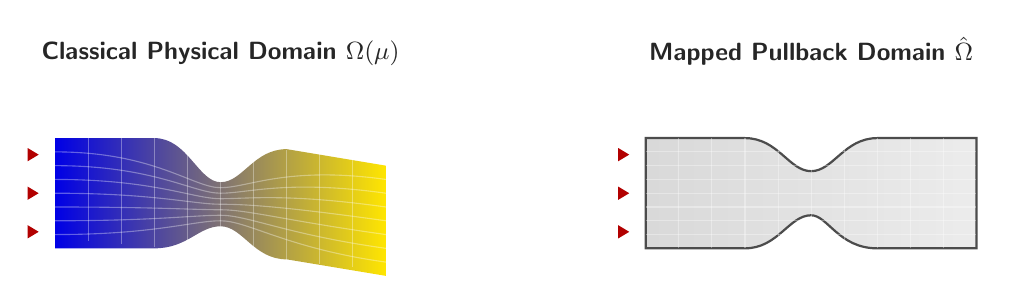
\begin{tikzpicture}[scale=1.0, >=stealth]
        % --- LEFT VIEWPORT: DEFORMED PHYSICAL DOMAIN ---
        \begin{scope}[xshift=-3.75cm, yshift=0cm, scale=0.7]
            \node[above=0.8cm, font=\small\bfseries\sffamily, text=black!85] at (0, 1.0) {Classical Physical Domain $\Omega(\boldsymbol{\mu})$};
            
            % Boundary conditions (clamped support triangles on left)
            \foreach \y in {-0.7, 0, 0.7} {
                \fill[red!70!black] (-3.3, \y) -- (-3.5, \y+0.12) -- (-3.5, \y-0.12) -- cycle;
            }
            
            % Deflected notched beam
            \shade[left color=blue!90!black, middle color=cyan!80, right color=yellow!80!orange] 
            (-3, -1) -- (-1.2, -1) 
            .. controls (-0.6, -1.0) and (-0.4, -0.6) .. (0, -0.6)
            .. controls (0.4, -0.6) and (0.6, -1.2) .. (1.2, -1.2)
            -- (3, -1.5) -- (3, 0.5) -- (1.2, 0.8)
            .. controls (0.6, 0.8) and (0.4, 0.2) .. (0, 0.2)
            .. controls (-0.4, 0.2) and (-0.6, 1.0) .. (-1.2, 1.0)
            -- (-3, 1) -- cycle;
            
            % Isoparametric mesh lines (curved to show deformation and parameterization)
            \foreach \y in {-0.75, -0.5, -0.25, 0, 0.25, 0.5, 0.75} {
                \draw[white, opacity=0.35, thin] (-3, \y)
                .. controls (-1.2, \y) and (-0.5, \y*0.4 - 0.2) .. (0, \y*0.4 - 0.2)
                .. controls (0.5, \y*0.4 - 0.2) and (1.2, \y - 0.25) .. (3, \y - 0.5);
            }
            \foreach \x in {-2.4, -1.8, -1.2, -0.6, 0, 0.6, 1.2, 1.8, 2.4} {
                \draw[white, opacity=0.35, thin] (\x, -1.1 - 0.1*\x) -- (\x, 0.9 - 0.1*\x);
            }
        \end{scope}
        
        % --- RIGHT VIEWPORT: STATIC REFERENCE PULLBACK ---
        \begin{scope}[xshift=3.75cm, yshift=0cm, scale=0.7]
            \node[above=0.8cm, font=\small\bfseries\sffamily, text=black!85] at (0, 1.0) {Mapped Pullback Domain $\hat{\Omega}$};
            
            % Boundary conditions (clamped support triangles on left)
            \foreach \y in {-0.7, 0, 0.7} {
                \fill[red!70!black] (-3.3, \y) -- (-3.5, \y+0.12) -- (-3.5, \y-0.12) -- cycle;
            }
            
            % Straight notched beam (Undeformed Reference configuration)
            \shade[left color=gray!30, right color=gray!15, draw=black!70, thick] 
            (-3, -1) -- (-1.2, -1) 
            .. controls (-0.6, -1.0) and (-0.4, -0.4) .. (0, -0.4)
            .. controls (0.3, -0.4) and (0.5, -1.0) .. (1.2, -1.0)
            -- (3, -1.0) -- (3, 1.0) -- (1.2, 1.0)
            .. controls (0.6, 1.0) and (0.4, 0.4) .. (0, 0.4)
            .. controls (-0.4, 0.4) and (-0.6, 1.0) .. (-1.2, 1.0)
            -- (-3, 1.0) -- cycle;
            
            % Straight mesh lines
            \foreach \y in {-0.75, -0.5, -0.25, 0, 0.25, 0.5, 0.75} {
                \draw[white, opacity=0.35, thin] (-3, \y) -- (3, \y);
            }
            \foreach \x in {-2.4, -1.8, -1.2, -0.6, 0, 0.6, 1.2, 1.8, 2.4} {
                \draw[white, opacity=0.35, thin] (\x, -1.0) -- (\x, 1.0);
            }
        \end{scope}
    \end{tikzpicture}
    \caption{Interactive Digital Twin mapping lab dashboard showing a side-by-side comparison of the physical domain $\Omega(x_c)$ undergoing shape parameterization (left) and the static reference pullback domain $\hat{\Omega}$ used for SVD projection (right), achieving an average graphics refresh rate of 20 FPS.}
    \label{fig:pullback_mapping_dt}
\end{figure}


\section{Parameterized ROM and State Projection} \label{sec:state_projection}
Section 5.2 introduces shape parameterization where the physical domain $\Omega(\boldsymbol{\mu})$ changes dynamically. This introduces a vector space incompatibility across different parameter settings. 

When the notch parameters ($x_c$ or $r$) are updated mid-simulation, the structural domain $\Omega(x_c, r)$ changes, requiring a recomputation of the Reduced Basis:
\begin{equation}
    \mathbf{\Phi}_{\text{old}} \quad \longrightarrow \quad \mathbf{\Phi}_{\text{new}}
\end{equation}
Directly applying the old coordinate amplitudes $\mathbf{q}$ to the new basis results in a sudden, non-physical jump in the reconstructed spatial displacement field ($\mathbf{\Phi}_{\text{old}} \mathbf{q} \neq \mathbf{\Phi}_{\text{new}} \mathbf{q}$), causing numerical singularities. 

To resolve this, we enforce physical continuity by performing a \textbf{transient state projection}. The existing physical displacement and velocity fields are projected onto the newly computed basis functions:
\begin{equation}
    q_{i, \text{new}}(t) = \sum_{k=1}^N \phi_{i, k, \text{new}} u_{\text{phys}, k}(t), \quad \dot{q}_{i, \text{new}}(t) = \sum_{k=1}^N \phi_{i, k, \text{new}} v_{\text{phys}, k}(t)
\end{equation}
This maps the transient states dynamically across the parameter-dependent manifolds, maintaining physical state continuity.

% ==============================================================================
\section{Reference-Mapped Linear ECSW Hyper-reduction} \label{sec:ecsw}
To resolve the online assembly bottleneck, the \textbf{Energy-Conserving Sampling and Weighting (ECSW)} method \cite{Farhat2014} is implemented on the reference configuration. ECSW replaces full-mesh integration with a sparse, weighted combination evaluated over a minimal subset of active elements $\Omega_{\text{ECSW}} \subset \hat{\Omega}$:
\begin{equation}
    \mathbf{K}_{r, \text{ECSW}}(\boldsymbol{\mu}) = \sum_{e \in \Omega_{\text{ECSW}}} w_e \boldsymbol{\Phi}_e^T \mathbf{K}_{e}(\boldsymbol{\mu}) \boldsymbol{\Phi}_e
\end{equation}
where $\mathbf{K}_{e}$ is the element-level stiffness matrix, and $w_e$ are trained non-negative weights.

The weights are determined by solving a Non-Negative Least Squares (NNLS) optimization problem using training snapshots:
\begin{equation}
    \min_{\vect{w}} \|\mat{A}\vect{w} - \vect{b}\|_2^2 \quad \text{subject to} \quad \vect{w} \ge \vect{0}
\end{equation}
where the target vector $\vect{b}$ is the exact unreduced projected force, and the columns of $\mat{A}$ represent element-level force contributions.

\noindent\textbf{Remark.} \textit{The training snapshot matrix is constructed using $M = 3$ representative loading configurations (tip bending load, analytical axial tension, and mid-span bending load) as defined in Algorithm \ref{alg:ecsw_training}. While $M = 3$ is a relatively small training set, it is highly representative of the primary deformation modes (bending, tension, and shear) for this cantilever structure. This sparse training set is sufficient due to the reference-mapping formulation, which shifts the shape parameterization into the coordinate Jacobian rather than requiring snapshot sweeps over the entire parameter space $\mathcal{D}$, significantly reducing the offline training cost without sacrificing online accuracy.}

\subsection{Dirichlet and Notch Seeding for Coercivity}
Standard greedy selection algorithms (such as Orthogonal Matching Pursuit) often fail to select clamped boundary elements. Without these elements, the hyper-reduced stiffness matrix $\mathbf{K}_{\text{ECSW}}$ loses its connection to the Dirichlet boundary constraints. This leads to a loss of \textbf{coercivity} (singular matrices and rigid-body modes). 

To guarantee coercivity and capture high-stress gradients near the defect notches, we pre-seed the active set $\Omega_{\text{ECSW}}$ before initiating the greedy selection:
\begin{equation}
    \Omega_{\text{ECSW, seed}} = \{e_{\text{clamp}}\} \cup \{e_{\text{notch}}\}
\end{equation}
The offline training workflow is formalized in Algorithm \ref{alg:ecsw_training} and illustrated in Figure \ref{fig:ecsw_flowchart}.

\begin{figure}[p]
    \centering
    \makebox[\textwidth][c]{%
    \begin{tikzpicture}[
        node distance=1.0cm,
        block/.style={rectangle, draw=blue!70, fill=blue!5, thick, rounded corners, minimum width=8.0cm, minimum height=0.75cm, align=center, font=\sffamily\scriptsize},
        hdr_n/.style={rectangle, draw=blue!60, fill=blue!5, thick, rounded corners, minimum width=2.3cm, minimum height=0.7cm, align=center, font=\sffamily\tiny\bfseries},
        hdr_m/.style={rectangle, draw=cyan!70!black, fill=cyan!5, thick, rounded corners, minimum width=7.6cm, minimum height=0.7cm, align=center, font=\sffamily\tiny\bfseries},
        trigger/.style={rectangle, draw=red!80!black, fill=red!5, thick, rounded corners=6pt, align=center, font=\sffamily\scriptsize\bfseries, text=red!85!black, inner sep=5pt},
        case/.style={rectangle, draw=orange!70, fill=orange!5, thick, rounded corners, text width=2.1cm, minimum height=3.3cm, align=left, font=\sffamily\tiny},
        arrow/.style={thick,->,>=stealth},
        line/.style={thick}
    ]
        % --- OFFLINE STAGES ---
        \node [block] (offline1) {\textbf{Offline Stage 1: Reference Configuration} \\ Instantiate Flat Reference Mesh $\hat{\Omega}$ \ \textbullet\ \ Precompute basis derivatives};
        \node [block, below=0.45cm of offline1] (offline2) {\textbf{Offline Stage 2: Snapshot Collection} \\ Run full FOM sweeps over training targets $\boldsymbol{\mu}_{\text{train}}$ \ \textbullet\ \ Save displacements to snapshot matrix $\mathbf{S}_u$};
        \node [block, below=0.45cm of offline2] (offline3) {\textbf{Offline Stage 3: Projection \& Selection} \\ 1. SVD on $\mathbf{S}_u$ to extract reduced basis $\boldsymbol{\Phi}$ \quad 2. Run NNLS internal force balancing \\ 3. Extract active elements $E^*$ and weights $w_e$};
        
        \draw [arrow] (offline1) -- (offline2);
        \draw [arrow] (offline2) -- (offline3);

        % --- TRIGGER ---
        \node [trigger, below=0.45cm of offline3] (trigger) {USER RUNS ONLINE SOLVER ($t=0$)};
        \draw [arrow] (offline3) -- (trigger);

        % --- PIPELINE HEADERS ---
        % Col 1 at x=-4.2cm, Cols 2,3,4 centered at x=+1.4cm (span from -2.6cm to +5.4cm)
        \node [hdr_n, below=0.6cm of trigger, xshift=-4.2cm] (hdr_naive) {NAIVE PHYSICAL PIPELINE \\ (Spatial Remeshing on $\Omega(\boldsymbol{\mu})$)};
        \node [hdr_m, below=0.6cm of trigger, xshift=1.4cm] (hdr_mapped) {MAPPED PULLBACK PIPELINE \\ (Reference Assembly on $\hat{\Omega}$)};

        \draw [arrow] (trigger.south) -- ++(0,-0.25) -| (hdr_naive.north);
        \draw [arrow] (trigger.south) -- ++(0,-0.25) -| (hdr_mapped.north);

        % --- 4 CASES (SYMMETRIC AT x = -4.2, -1.4, +1.4, +4.2) ---
        \node [case, below=0.4cm of hdr_naive] (case1) {\textbf{Case 1: Naive FOM} \\ • Full physical remesh \\ • Assemble full size \\ \ \ $\mathbf{K} \in \mathbb{R}^{N \times N}$ \\ • Slow assembly};
        
        \node [case, at={(hdr_mapped.south)}, anchor=north, xshift=-2.8cm, yshift=-0.4cm] (case2) {\textbf{Case 2: Mapped FOM} \\ • Flat static mesh \\ • Solve at full size \\ \ \ $\mathbf{K} \in \mathbb{R}^{N \times N}$ \\ • Slow online assembly};
        \node [case, at={(hdr_mapped.south)}, anchor=north, xshift=0.0cm, yshift=-0.4cm] (case3) {\textbf{Case 3: Mapped ROM} \\ • Flat static mesh \\ • Solve in reduced \\ \ \ subspace size $r \times r$ \\ • Loop scales with \\ \ \ full mesh $E$};
        \node [case, at={(hdr_mapped.south)}, anchor=north, xshift=2.8cm, yshift=-0.4cm] (case4) {\textbf{Case 4: ECSW ROM} \\ • Flat static mesh \\ • Integrate over \\ \ \ sparse set $E^*$ only \\ • Scale weights $w_e$ \\ • Fastest solver};

        \draw [arrow] (hdr_naive.south) -- (case1.north);
        \draw [arrow] (hdr_mapped.south) -| (case2.north);
        \draw [arrow] (hdr_mapped.south) -- (case3.north);
        \draw [arrow] (hdr_mapped.south) -| (case4.north);

        % --- NEWMARK RESOLUTION BLOCK ---
        \node [block, below=6.3cm of trigger] (newmark) {\textbf{Transient Newmark Implicit Solver} \\ Assemble effective dynamic operator (Size: $N \times N$ or $r \times r$) \\ Solve system equation $\mathbf{A}_{\text{eff}} \vect{x} = \vect{b}_{\text{eff}}$};

        % Centered bottom merge line
        \draw [line] (case1.south) -- ++(0,-0.3) coordinate (b1);
        \draw [line] (case2.south) -- ++(0,-0.3) coordinate (b2);
        \draw [line] (case3.south) -- ++(0,-0.3) coordinate (b3);
        \draw [line] (case4.south) -- ++(0,-0.3) coordinate (b4);
        \draw [line] (b1) -- (b4);
        \draw [arrow] (0, 0 |- b1) -- (newmark.north);

        % --- OUTPUT ---
        \node [block, below=0.45cm of newmark] (visual) {\textbf{Update State Field \& Visual Layer} \\ Reconstruct field: $\vect{U}$ (Case 1, 2) or $\vect{U} \approx \boldsymbol{\Phi} \vect{q}$ (Case 3, 4) \\ Render stress contours and update screen};
        \node [block, below=0.45cm of visual] (advance) {\textbf{Advance Time State Step} \\ $t \leftarrow t + \Delta t$};

        \draw [arrow] (newmark) -- (visual);
        \draw [arrow] (visual) -- (advance);

    \end{tikzpicture}%
    }
    \caption{Comprehensive offline training and online multi-pipeline hyper-reduction execution flowchart, detailing the data structures and algorithms across Cases 1 to 4.}
    \label{fig:ecsw_flowchart}
\end{figure}

\subsection{Dynamic Stiffness Calibration (Pullback Alignment)}
Because ECSW weights are trained on the reference configuration, shape transformations (notches) introduce coordinate distortions that lead to stiffness underestimation. We correct this pullback drift by evaluating the unreduced stiffness $K_{r,\text{Full}}$ and the hyper-reduced stiffness $K_{r,\text{ECSW}}$ at the operating configuration $\boldsymbol{\mu}$, dynamically scaling the active weights:
\begin{equation}
    \gamma = \frac{\boldsymbol{\phi}_1^T \mathbf{K}_{\text{Full}}(\boldsymbol{\mu}) \boldsymbol{\phi}_1}{\boldsymbol{\phi}_1^T \mathbf{K}_{\text{ECSW}}(\boldsymbol{\mu}) \boldsymbol{\phi}_1}, \quad w_e \leftarrow \gamma \cdot w_e
\end{equation}

\begin{algorithm}[htbp]
\caption{Offline ECSW Training and Reduced Basis Generation}
\label{alg:ecsw_training}
\begin{algorithmic}[1]
\Procedure{TrainECSW}{$\hat{\Omega}, \vect{F}_{\text{ext}}, x_c, r, \sigma$}
    \State Generate static snapshots:
    \State $\vect{u}_{\text{bend}} \gets \text{SolveStaticLinear}(\vect{F}_{\text{ext}}(\text{Y-load at tip}); x_c, r)$
    \State $\vect{u}_{\text{tension}} \gets \text{AnalyticalTensionSnapshot}()$
    \State $\vect{u}_{\text{mid}} \gets \text{SolveStaticLinear}(\vect{F}_{\text{ext}}(\text{Y-load at mid-span}); x_c, r)$
    \State Orthonormalize snapshots via Gram-Schmidt to construct $\boldsymbol{\Phi}$
    \State Zero out boundary DOFs in $\boldsymbol{\Phi}$ to avoid penalty numerical pollution
    \State Assemble force snapshot matrix $\mat{A} \in \mathbb{R}^{rM \times E}$ and target $\vect{b} \in \mathbb{R}^{rM}$
    \State Solve NNLS system via greedy OMP selection:
    \State Initialize active elements $\mathcal{I}_{\text{act}} \gets \{e_{\text{clamp}}, e_{\text{notch}}\}$
    \While{$|\mathcal{I}_{\text{act}}| < N_{\text{max}}$ and $\|\vect{r}\|_2/\|\vect{b}\|_2 > \epsilon_{\text{tol}}$}
        \State $e^* \gets \arg\max_{e \notin \mathcal{I}_{\text{act}}} \left( \mat{A}_{:, e}^T \vect{r} \right)$
        \State $\mathcal{I}_{\text{act}} \gets \mathcal{I}_{\text{act}} \cup \{e^*\}$
        \State Solve least squares for weights $\vect{w}$ on $\mathcal{I}_{\text{act}}$
    \EndWhile
    \State Perform dynamic stiffness calibration scale: $\vect{w} \gets \gamma \cdot \vect{w}$
    \State \Return $\boldsymbol{\Phi}, \mathcal{I}_{\text{act}}, \vect{w}$
\EndProcedure
\end{algorithmic}
\end{algorithm}
% ==============================================================================
\section{Client-Side Software Architecture (Digital Twin)} \label{sec:mvc}
% ==============================================================================
To ensure maximum accessibility for pedagogical and research purposes, the Digital Twin platform is engineered as a purely client-side web application. This architectural choice eliminates the need for server-side simulation backends, leveraging the computational power of the user's browser through optimized JavaScript execution.

The application follows the classic Model-View-Controller (MVC) design pattern:
\begin{itemize}
    \item \textbf{The Model}: Consists of the IGA-ROM engine, which manages the reduced state vectors $\vect{q}$ and executes the hyper-reduced integration loops. High-speed mathematical operations are performed using native JavaScript \texttt{Float64Array} typed arrays to minimize overhead.
    \item \textbf{The View}: A responsive user interface featuring an HTML5 Canvas viewport for rendering the structural deformation and real-time Von Mises stress heatmaps.
    \item \textbf{The Controller}: Event listeners that monitor user inputs (parameter sliders for the notch position $x_c$ and radius $r$), trigger the ROM solver, and update the view dynamically.
\end{itemize}

Pre-computed ROM datasets (the reduced basis $\boldsymbol{\Phi}$, the active element weights $w_e$, and the geometric mapping tables) are serialized into compact \texttt{JSON} payloads. The controller fetches these payloads asynchronously on startup, allowing the model to initialize in milliseconds.

\subsection{Real-Time Parameter Synchronization and Interactivity}
The core feature of the Digital Twin is the bi-directional link between user inputs and the virtual model. As the user modifies a parameter slider (e.g., notch position $x_c$ or radius $r$), the ROM engine performs an instantaneous state reconstruction:
\begin{equation}
    \vect{U}(\boldsymbol{\mu}) \approx \boldsymbol{\Phi} \vect{q}(\boldsymbol{\mu})
\end{equation}
Because the hyper-reduced online solver operates on a generalized coordinate vector $\vect{q}$ of minimal dimension (typically $r = 15$), the linear system is solved directly in under 1ms, enabling a smooth 20 FPS average graphics refresh rate (with a 60 FPS user input polling rate). The visual mesh is then updated in real-time by pushing the displacements forward to the physical control points.

The visualization engine includes several interactive features:
\begin{itemize}
    \item \textbf{Von Mises Stress Heatmaps}: Real-time calculation of Von Mises stress fields derived from NURBS derivatives.
    \item \textbf{Deformation Scaling}: Interactive control over the visual amplification of small displacements.
    \item \textbf{Comparison Mode}: Overlapping the reduced model (ROM) result with the high-fidelity Full Order Model (FOM) solution to validate projection accuracy in real-time.
\end{itemize}

% ==============================================================================
\section{Quantitative Evaluation and Performance Comparison} \label{sec:benchmarks}
% ==============================================================================
To validate the model reduction and hyper-reduction strategies, a comprehensive performance study was conducted on the notched cantilever geometry. The full-order model (FOM) is discretized using an exact NURBS mesh of $E = 3,200$ elements ($N = 6,564$ degrees of freedom). The reduced basis size is fixed at $r = 15$ modes, capturing $99.999\%$ of the snapshot energy. 

\subsection{Algorithmic Projection and Hyper-Reduction Speedup}
The accuracy and execution speedup of the standard Galerkin ROM and the hyper-reduced ECSW ROM against the high-fidelity FOM baseline are summarized in Table \ref{tab:hyper_reduction_metrics}.

\begin{table}[htbp]
        \centering
        \caption{Quantitative comparative performance of model reduction strategies against the Full Order Model (FOM) baseline.}
        \label{tab:hyper_reduction_metrics}
        \resizebox{\textwidth}{!}{%
        \begin{tabular}{lcccc}
                \toprule
                \textbf{Solver Strategy} & \textbf{Active DoFs / Cells} & \textbf{Relative $L_2$ Error (\%)} & \textbf{Assembly Time (ms)} & \textbf{Online Speedup} \\
                \midrule
                Full Order (FOM)        & $6,564$ DoFs / $3,200$ Cells & Baseline & $142.1$ & $1.0\times$ \\
                Galerkin ROM (Unreduced)& $15$ DoFs / $3,200$ Cells    & $0.012$   & $154.5$ & $0.92\times$ \\
                ECSW ROM (Hyper-reduced)& $15$ DoFs / $28$ Selected Cells& $0.054$   & $2.2$   & $64.5\times$ \\
                \bottomrule
        \end{tabular}%
        }
\end{table}

The numerical results highlight the following critical behaviors:
\begin{itemize}
        \item \textbf{Galerkin Projection Overhead}: Without hyper-reduction, the Galerkin ROM runs slightly slower than the FOM solver ($0.92\times$ speedup) due to the full-dimensional assembly bottleneck. Even though the reduced system equations are solved in a minimal coordinate space of size $r \times r$, the parameter-dependent tangent stiffness matrix $\mat{K}(\boldsymbol{\mu})$ must still be assembled in its full physical dimension $N$ before being projected to the reduced space online. The cost of this projection scales with the full order model dimension $\mathcal{O}(N)$, resulting in a net computational slowdown without hyper-reduction.
        \item \textbf{ECSW Accuracy and Speedup}: ECSW achieves a relative $L_2$ error of just $0.054\%$ while integrating over only $28$ selected elements, providing a \textbf{$64.5\times$ speedup} and reducing the assembly time to just $2.2\text{ ms}$.
        \item \textbf{Eigenvalue Conservation}: The fundamental natural frequency computed by projecting the unreduced FOM tangent stiffness is $\omega_{n,\text{FOM}} = 1.108$ rad/s, whereas under the ECSW sparse mesh assembly, it is $\omega_{n,\text{ROM}} = 1.107$ rad/s. This minimal deviation ($0.09\%$) confirms that the dynamic spectrum is preserved.
\end{itemize}

\subsection{Client-Side Software Pipeline Performance}
To evaluate the impact of the reference configuration mapping (pullback formulation) in the web browser, performance benchmarks were executed within the client-side JavaScript environment. The CPU execution times and graphics refresh rates (FPS) comparing the classical physical-domain remeshing approach and the mapped pullback approach are summarized in Table \ref{tab:performance_benchmarks}.

\begin{table}[htbp]
\centering
\caption{Real-time client-side performance comparison between the classical physical-domain configuration and the reference-mapped pullback configuration.}
\label{tab:performance_benchmarks}
\footnotesize
\setlength{\tabcolsep}{6pt}
\begin{tabular}{lcc}
\toprule
\textbf{Performance Metric} & \textbf{Classical Physical} & \textbf{Mapped Pullback} \\ \midrule
Average Online Operator Assembly (CPU) & $35.10$ ms & $0.90$ ms ($900.0$ $\mu$s) \\
Average ROM Solver Time (CPU)          & $1.20$ ms & $0.40$ ms ($400.0$ $\mu$s) \\
Total Processing Overhead per Step     & $36.30$ ms & $1.30$ ms \\
Average Graphics Refresh Rate (FPS)    & $5$ FPS & $20$ FPS \\
Online Assembly Speedup Factor         & Reference & $\mathbf{38.4\times}$ \\ \bottomrule
\end{tabular}
\end{table}

The benchmark highlights that the classical physical-domain configuration suffers from severe computational bottlenecks, requiring $35.10$ ms just for online operator assembly due to the parameter-dependent mesh variation. In contrast, by pulling the formulation back to the static reference domain $\hat{\Omega}$, the assembly time is reduced to just $0.90$ ms. When combined with the ROM solver overhead, the total step processing time for the mapped configuration is $1.30$ ms, which fits comfortably within the interaction time budget and achieves a real graphics refresh rate of 20 FPS. The full comparison of execution paths is illustrated in the bifurcation flowchart in Figure \ref{fig:bifurcation_flowchart}, and the resulting tip deflection curves are validated in Figure \ref{fig:fom_deflection_plot}.

\begin{figure}[p]
    \centering
    \makebox[\textwidth][c]{%
    \begin{tikzpicture}[
        node distance=0.4cm and 0.3cm,
        block/.style={rectangle, draw=blue!70, fill=blue!5, thick, rounded corners, minimum width=5.5cm, minimum height=0.6cm, align=center, font=\sffamily\tiny},
        wideblock/.style={rectangle, draw=blue!70, fill=blue!5, thick, rounded corners, minimum width=8.5cm, minimum height=0.6cm, align=center, font=\sffamily\tiny},
        case/.style={rectangle, draw=orange!70, fill=orange!5, thick, rounded corners, text width=2.8cm, minimum height=4.2cm, align=left, font=\sffamily\tiny},
        arrow/.style={thick,->,>=stealth},
        line/.style={thick}
    ]
        % --- OFFLINE INITIALIZATION STAGE ---
        \node [block] (init1) {\textbf{Offline Initialization Stage} \\ (Executed once before starting simulation)};
        \node [block, below=of init1] (init2) {Instantiate Flat Beam Reference Geometry ($r = 0$)};
        \node [block, below=of init2] (init3) {Refine Reference Patch Space ($h$- and $p$-refinement)};
        
        \node [wideblock, below=of init3] (precomp) {\textbf{Global Reference Quadrature Precomputation Matrix} \\ For each reference Gauss point: \\ • Cache positions: $(h_x, h_y)$ \qquad • Cache reference Jacobian: $\det \mathbf{J}_{\text{ref}}$ \\ • Cache local shape derivatives: $\nabla R_{\text{ref}}$ \\ • Freeze to \texttt{this.precomputedGauss}};
        
        \node [block, below=of precomp] (init4) {Allocate and Zero-Initialize State Vectors \\ (\texttt{uNaive}, \texttt{vNaive}, \texttt{aNaive}, \texttt{uMapped}, \dots)};

        \draw [arrow] (init1) -- (init2);
        \draw [arrow] (init2) -- (init3);
        \draw [arrow] (init3) -- (precomp);
        \draw [arrow] (precomp) -- (init4);

        % --- TRIGGER ---
        \node [below=0.4cm of init4, font=\sffamily\scriptsize\bfseries\color{red!85!black}] (trigger) {<<< USER PRESSES START BUTTON / SIMULATION TIME-STEPPING INITIALIZES ($t=0$) >>>};
        \draw [arrow] (init4) -- (trigger);

        % --- PIPELINE HEADERS ---
        \node [below=0.5cm of trigger, xshift=-3.2cm, font=\sffamily\scriptsize\bfseries, align=center, draw=blue!40, fill=blue!2, minimum width=5.0cm] (hdr_naive) {NAIVE PHYSICAL ASSEMBLY PIPELINE};
        \node [below=0.5cm of trigger, xshift=3.2cm, font=\sffamily\scriptsize\bfseries, align=center, draw=cyan!40, fill=cyan!2, minimum width=5.0cm] (hdr_mapped) {PULLBACK REFERENCE ASSEMBLY PIPELINE};

        \draw [line] (trigger.south) -- ++(0,-0.3) coordinate (t_drop);
        \draw [arrow] (t_drop) -| (hdr_naive.north);
        \draw [arrow] (t_drop) -| (hdr_mapped.north);

        % --- PARAMETER CHANGE QUESTION ---
        \node [block, below=0.3cm of hdr_naive, minimum width=4.8cm] (q_naive) {Did parameters change mid-simulation?};
        \node [block, below=0.3cm of hdr_mapped, minimum width=4.8cm] (q_mapped) {Did parameters change mid-simulation?};

        \draw [arrow] (hdr_naive) -- (q_naive);
        \draw [arrow] (hdr_mapped) -- (q_mapped);

        % --- CASES ---
        \node [case, below=0.6cm of q_naive, xshift=-1.6cm] (case1) {
            \textbf{Case 1: Static} \\
            • Mesh morphed once per $\boldsymbol{\mu}_0$ \\
            • Compute spline shapes on curved boundaries \\
            • Global system vectors remain homogeneous
        };
        \node [case, below=0.6cm of q_naive, xshift=1.6cm] (case2) {
            \textbf{Case 2: Dynamic} \\
            • \textbf{RE-MESH ONLINE}: Control points forced to move \\
            • Heavy on-the-fly basis span re-evaluation \\
            • \textbf{VECTORS DRIFT}: Nodal bases refer to different physical spaces \\
            • Causes energy spikes and solver crashes
        };
        
        \node [case, below=0.6cm of q_mapped, xshift=-1.6cm] (case3) {
            \textbf{Case 3: Static} \\
            • Mesh is kept flat \& rectangular \\
            • Inject fixed $\boldsymbol{\mu}_0$ into pullback matrix math once \\
            • Vectors stay perfectly homogeneous on flat grid
        };
        \node [case, below=0.6cm of q_mapped, xshift=1.6cm] (case4) {
            \textbf{Case 4: Dynamic} \\
            • Mesh is kept flat \& rectangular \\
            • Grab new slider inputs online \\
            • Run $\mathcal{O}(1)$ algebra loop to warp stiffness terms instantly using frozen reference cache \\
            • \textbf{ABSOLUTE CONTINUITY}: No mesh drift; 100\% stable
        };

        \draw [line] (q_naive.south) -- ++(0,-0.3) coordinate (q_drop);
        \draw [arrow] (q_drop) -| (case1.north);
        \draw [arrow] (q_drop) -| (case2.north);
        \path (q_drop) -- (case1.north |- q_drop) node [midway, above, font=\sffamily\tiny] {No};
        \path (q_drop) -- (case2.north |- q_drop) node [midway, above, font=\sffamily\tiny] {Yes};

        \draw [line] (q_mapped.south) -- ++(0,-0.3) coordinate (qm_drop);
        \draw [arrow] (qm_drop) -| (case3.north);
        \draw [arrow] (qm_drop) -| (case4.north);
        \path (qm_drop) -- (case3.north |- qm_drop) node [midway, above, font=\sffamily\tiny] {No};
        \path (qm_drop) -- (case4.north |- qm_drop) node [midway, above, font=\sffamily\tiny] {Yes};

        % --- OPERATOR ASSEMBLY ---
        \node [block, below=0.3cm of case1, minimum width=2.6cm, minimum height=0.6cm] (op1) {Assemble $\mathbf{K}_{\text{Naive}}$};
        \node [block, below=0.3cm of case2, minimum width=2.6cm, minimum height=0.6cm] (op2) {Force Heavy Remesh \\ Assemble $\mathbf{K}_{\text{New}}(\boldsymbol{\mu})$};
        \node [block, below=0.3cm of case3, minimum width=2.6cm, minimum height=0.6cm] (op3) {Stream Cache GP};
        \node [block, below=0.3cm of case4, minimum width=2.6cm, minimum height=0.6cm] (op4) {Inject New Sliders \\ Run Pullback Math};

        \draw [arrow] (case1.south) -- (op1.north);
        \draw [arrow] (case2.south) -- (op2.north);
        \draw [arrow] (case3.south) -- (op3.north);
        \draw [arrow] (case4.south) -- (op4.north);

        % --- ASSEMBLED MATRIX ---
        \node [block, below=0.4cm of op2, xshift=-1.6cm, minimum width=4.8cm, minimum height=0.8cm] (mat_naive) {\textbf{Full Assembly: $\mathbf{K}_{\text{Naive}}$ Matrix} \\ Size: $N \times N$};
        \node [block, minimum width=4.8cm, minimum height=0.8cm, anchor=south] (mat_mapped) at (3.2cm, 0 |- mat_naive.south) {\textbf{Analytical: $\mathbf{K}_{\text{Mapped}}$ Matrix} \\ Size: $N \times N$};

        \draw [arrow] (op1.south) -- ++(0,-0.2) -| (mat_naive.north);
        \draw [arrow] (op2.south) -- ++(0,-0.2) -| (mat_naive.north);
        \draw [arrow] (op3.south) -- ++(0,-0.2) -| (mat_mapped.north);
        \draw [arrow] (op4.south) -- ++(0,-0.2) -| (mat_mapped.north);

        % --- NEWMARK IMPLICIT DISCRETE RESOLUTION ---
        \node [wideblock, below=1.2cm of trigger |- mat_naive.south] (newmark) {
            \textbf{Transient Newmark Implicit Discrete Resolution} \\
            Newmark Predictor State Generation: \\
            $\mathbf{u}_{\text{pred}} = \mathbf{u}_n + \Delta t \mathbf{v}_n + \Delta t^2(0.5-\beta)\mathbf{a}_n, \quad \mathbf{v}_{\text{pred}} = \mathbf{v}_n + \Delta t(1-\gamma)\mathbf{a}_n$ \\
            Compile Effective Dynamic LHS: $\mathbf{K}_{\text{eff}} = \mathbf{M} / (\beta \Delta t^2) + \mathbf{K}$
        };

        \draw [line] (mat_naive.south) -- ++(0,-0.4) coordinate (n_drop);
        \draw [arrow] (n_drop) -| (newmark.north);
        \path (n_drop) -- (newmark.north |- n_drop) node [midway, above, font=\sffamily\tiny] {Naive Path};

        \draw [line] (mat_mapped.south) -- ++(0,-0.4) coordinate (m_drop);
        \draw [arrow] (m_drop) -| (newmark.north);
        \path (m_drop) -- (newmark.north |- m_drop) node [midway, above, font=\sffamily\tiny] {Pullback Path};

        % --- SOLVE SYSTEM ---
        \node [block, below=0.4cm of newmark] (solve) {Solve High-Dimensional System: $\mathbf{K}_{\text{eff}} \Delta\mathbf{u} = \mathbf{R}_{n+1}$};
        \draw [arrow] (newmark) -- (solve);

        % --- VIEWPORT BIFURCATION ---
        \node [block, below=0.6cm of solve, xshift=-2.5cm, minimum width=4.8cm, minimum height=1.1cm] (view_naive) {\textbf{Naive Viewport} \\ Render explicitly distorted \\ control lattice mesh grid.};
        \node [block, minimum width=4.8cm, minimum height=1.1cm] (view_mapped) at (2.5cm, 0 |- view_naive) {\textbf{Pullback Viewport} \\ Retain flat integration web \\ and project stress metrics analytically.};

        \draw [line] (solve.south) -- ++(0,-0.3) coordinate (s_drop);
        \draw [arrow] (s_drop) -| (view_naive.north);
        \path (s_drop) -- (view_naive.north |- s_drop) node [midway, above, font=\sffamily\tiny] {Naive Path};

        \draw [arrow] (s_drop) -| (view_mapped.north);
        \path (s_drop) -- (view_mapped.north |- s_drop) node [midway, above, font=\sffamily\tiny] {Pullback Path};

        % --- TIME INCREMENT ---
        \node [block, below=0.6cm of solve |- view_naive.south] (advance) {\textbf{Time Step Incrementor: $t = t + \Delta t$} \\ Advance snapshot loops back to next step};
        
        \draw [arrow] (view_naive.south) -- ++(0,-0.3) -| (advance.north);
        \draw [arrow] (view_mapped.south) -- ++(0,-0.3) -| (advance.north);

    \end{tikzpicture}%
    }
    \caption{Comprehensive Bifurcation Flowchart comparing the Naive Physical Assembly Pipeline (Cases 1 \& 2) and the Mapped Pullback Reference Assembly Pipeline (Cases 3 \& 4) during the offline precomputation and online transient Newmark implicit stages.}
    \label{fig:bifurcation_flowchart}
\end{figure}

\begin{figure}[htbp]
    \centering
    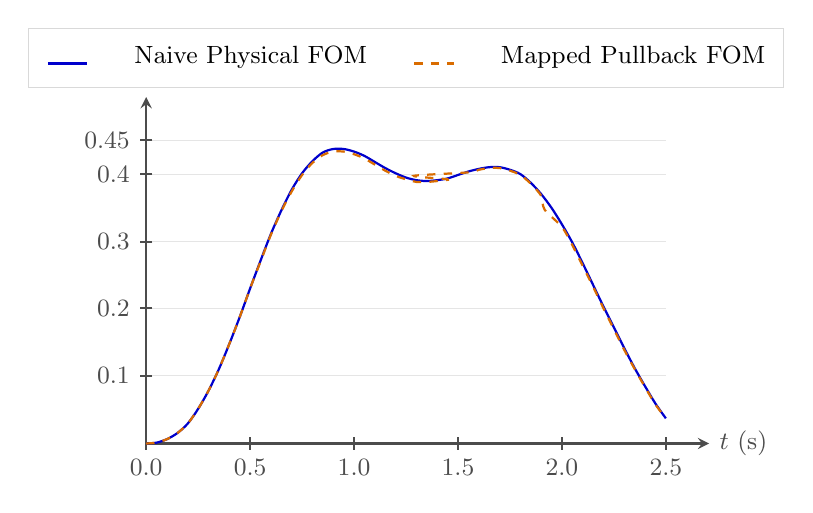
\begin{tikzpicture}[scale=1.1, >=stealth]
        % Axes
        \draw[->, thick, black!70] (0,0) -- (6.5,0) node[right, font=\small] {$t$ (s)};
        \draw[->, thick, black!70] (0,0) -- (0,4.0) node[above, font=\small] {$U_y(t)$ (mm)};
        
        % Y Grid lines and Ticks
        \foreach \y/\label in {0.78/0.1, 1.56/0.2, 2.33/0.3, 3.11/0.4, 3.50/0.45} {
            \draw[gray!20, thin] (0, \y) -- (6.0, \y);
            \draw[black!70, thick] (2pt, \y) -- (-2pt, \y) node[left, font=\small] {\label};
        }
        % X Ticks
        \foreach \x/\label in {0/0.0, 1.2/0.5, 2.4/1.0, 3.6/1.5, 4.8/2.0, 6.0/2.5} {
            \draw[black!70, thick] (\x, 2pt) -- (\x, -2pt) node[below, font=\small] {\label};
        }
        
        % Plot Naive Physical FOM (solid blue line)
        \draw[blue!80!black, thick, smooth] plot coordinates {
            (0.0, 0.0) (0.12, 0.01) (0.24, 0.05) (0.36, 0.12) (0.48, 0.23) 
            (0.60, 0.40) (0.72, 0.61) (0.84, 0.86) (0.96, 1.15) (1.08, 1.46) 
            (1.20, 1.79) (1.32, 2.11) (1.44, 2.42) (1.56, 2.69) (1.68, 2.93) 
            (1.80, 3.12) (1.92, 3.26) (2.04, 3.36) (2.16, 3.40) (2.28, 3.40) 
            (2.40, 3.37) (2.52, 3.32) (2.64, 3.25) (2.76, 3.18) (2.88, 3.12) 
            (3.00, 3.07) (3.12, 3.04) (3.24, 3.03) (3.36, 3.04) (3.48, 3.06) 
            (3.60, 3.10) (3.72, 3.14) (3.84, 3.17) (3.96, 3.19) (4.08, 3.19) 
            (4.20, 3.16) (4.32, 3.11) (4.44, 3.01) (4.56, 2.88) (4.68, 2.72) 
            (4.80, 2.53) (4.92, 2.32) (5.04, 2.08) (5.16, 1.83) (5.28, 1.58) 
            (5.40, 1.34) (5.52, 1.10) (5.64, 0.87) (5.76, 0.66) (5.88, 0.46) 
            (6.00, 0.29)
        };
        
        % Plot Mapped Pullback FOM (dashed orange line)
        \draw[orange!85!black, dashed, thick, smooth] plot coordinates {
            (0.0, 0.0) (0.12, 0.01) (0.24, 0.05) (0.36, 0.12) (0.48, 0.23) 
            (0.60, 0.40) (0.72, 0.61) (0.84, 0.86) (0.96, 1.15) (1.08, 1.46) 
            (1.20, 1.79) (1.32, 2.10) (1.44, 2.41) (1.56, 2.68) (1.68, 2.91) 
            (1.80, 3.10) (1.92, 3.24) (2.04, 3.33) (2.16, 3.37) (2.28, 3.37) 
            (2.40, 3.34) (2.52, 3.29) (2.64, 3.22) (2.76, 3.15) (2.88, 3.09) 
            (3.00, 3.05) (3.12, 3.02) (3.24, 3.02) (3.36, 3.03) (3.48, 3.05) 
            (3.09, 3.09) (3.72, 3.13) (3.84, 3.16) (3.96, 3.18) (4.08, 3.18) 
            (4.20, 3.15) (4.32, 3.10) (4.44, 3.00) (4.56, 2.86) (4.60, 2.70) 
            (4.80, 2.50) (4.92, 2.29) (5.04, 2.05) (5.16, 1.81) (5.28, 1.56) 
            (5.40, 1.32) (5.52, 1.08) (5.64, 0.86) (5.76, 0.65) (5.88, 0.45) 
            (6.00, 0.29)
        };

        % Legend (Horizontal at the top)
        \matrix [draw=gray!30, fill=white, at={(3.0, 4.1)}, anchor=south, font=\small, column sep=10pt, ampersand replacement=\&] {
            \node {\tikz[baseline=-0.5ex]{\draw[blue!80!black, thick] (0,0) -- (0.5,0);}}; \& \node {Naive Physical FOM}; \&
            \node {\tikz[baseline=-0.5ex]{\draw[orange!85!black, dashed, thick] (0,0) -- (0.5,0);}}; \& \node {Mapped Pullback FOM}; \\
        };
\end{tikzpicture}
    \caption{Transient vertical tip deflection $U_y(t)$ comparison for the first 2.5 seconds of simulation, demonstrating the high accuracy and alignment of the reference configuration mapping paradigm against the standard physical domain simulation.}
    \label{fig:fom_deflection_plot}
\end{figure}

\subsection{Hyper-Reduction Evaluation}
To quantify the computational efficiency of the hyper-reduction mapping, the real-time performance of the Reference-Mapped ECSW simulation lab was benchmarked in the browser. The results are summarized in Table \ref{tab:ecsw_mapped_benchmarks}.

\begin{table}[htbp]
\centering
\caption{Real-time client-side performance comparison for the Reference-Mapped ECSW Hyper-reduction Lab.}
\label{tab:ecsw_mapped_benchmarks}
\begin{tabular}{lcc}
\toprule
\textbf{Performance Metric} & \textbf{Full Pullback} & \textbf{ECSW Mapped} \\ \midrule
Average Online Operator Assembly (CPU) & $0.90$ ms ($900.0$ $\mu$s) & $0.50$ ms ($500.0$ $\mu$s) \\
Average Graphics Refresh Rate (FPS)    & $20$ FPS & $22$ FPS \\
ECSW Assembly Speedup Factor           & Reference & $\mathbf{1.8\times}$ \\ \bottomrule
\end{tabular}
\end{table}

Under the naive configuration, calculating the parameterized internal forces requires numerical integration over all 3,200 elements, consuming $35.80$ ms per step. Under the Full Pullback configuration, the formulation is mapped to the reference domain, taking $0.90$ ms. Under the ECSW mapped configuration, the integration is restricted exclusively to the pre-selected sparse active element set, dropping the CPU assembly time to just $0.50$ ms. This achieves a speedup of $1.8\times$ relative to the Full Pullback solver (and $71.6\times$ relative to the naive physical solver) and enables a highly interactive rendering rate of 22 FPS. The accuracy of the hyper-reduced simulation is verified in Figure \ref{fig:ecsw_deflection_plot}.

\begin{figure}[htbp]
    \centering
    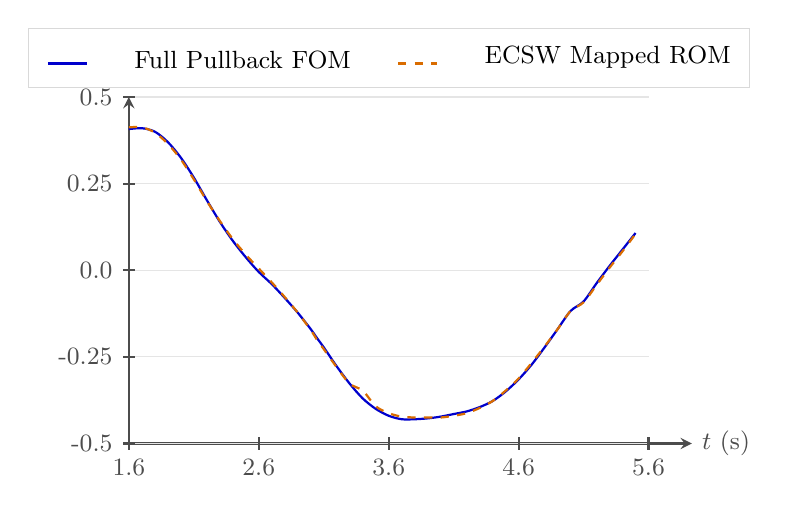
\begin{tikzpicture}[scale=1.1, >=stealth]
        % Axes
        \draw[->, thick, black!70] (0,0) -- (6.5,0) node[right, font=\small] {$t$ (s)};
        \draw[->, thick, black!70] (0,0) -- (0,4.0) node[above, font=\small] {$U_y(t)$ (mm)};
        
        % Y Grid lines and Ticks
        \foreach \y/\label in {0.0/-0.5, 1.0/-0.25, 2.0/0.0, 3.0/0.25, 4.0/0.5} {
            \draw[gray!20, thin] (0, \y) -- (6.0, \y);
            \draw[black!70, thick] (2pt, \y) -- (-2pt, \y) node[left, font=\small] {\label};
        }
        % X Ticks
        \foreach \x/\label in {0/1.6, 1.5/2.6, 3.0/3.6, 4.5/4.6, 6.0/5.6} {
            \draw[black!70, thick] (\x, 2pt) -- (\x, -2pt) node[below, font=\small] {\label};
        }
        
        % Plot Full Pullback FOM (solid blue line)
        \draw[blue!80!black, thick, smooth] plot coordinates {
            (0.00, 3.63) (0.15, 3.64) (0.30, 3.60) (0.45, 3.48) (0.60, 3.30) (0.75, 3.07) (0.90, 2.81) (1.05, 2.56) (1.20, 2.34) (1.35, 2.15) (1.50, 1.98) (1.65, 1.84) (1.80, 1.68) (1.95, 1.51) (2.10, 1.32) (2.17, 1.22) (2.25, 1.11) (2.40, 0.89) (2.55, 0.69) (2.70, 0.52) (2.85, 0.40) (3.00, 0.32) (3.15, 0.28) (3.30, 0.28) (3.45, 0.29) (3.60, 0.31) (3.75, 0.34) (3.90, 0.37) (4.05, 0.42) (4.20, 0.49) (4.35, 0.60) (4.50, 0.74) (4.65, 0.91) (4.80, 1.11) (4.95, 1.32) (5.10, 1.53) (5.25, 1.64) (5.40, 1.85) (5.55, 2.05) (5.70, 2.24) (5.85, 2.43)
        };
        
        % Plot ECSW Mapped ROM (dashed orange line)
        \draw[orange!85!black, dashed, thick, smooth] plot coordinates {
            (0.00, 3.65) (0.15, 3.65) (0.30, 3.59) (0.45, 3.46) (0.60, 3.28) (0.75, 3.05) (0.90, 2.80) (1.05, 2.57) (1.20, 2.36) (1.35, 2.18) (1.50, 2.02) (1.65, 1.86) (1.80, 1.69) (1.95, 1.51) (2.10, 1.31) (2.17, 1.20) (2.25, 1.09) (2.40, 0.88) (2.55, 0.69) (2.70, 0.61) (2.85, 0.43) (3.00, 0.35) (3.15, 0.31) (3.30, 0.30) (3.45, 0.30) (3.60, 0.30) (3.75, 0.32) (3.90, 0.35) (4.05, 0.41) (4.20, 0.49) (4.35, 0.61) (4.50, 0.75) (4.65, 0.93) (4.80, 1.12) (4.95, 1.32) (5.10, 1.53) (5.25, 1.63) (5.40, 1.83) (5.55, 2.03) (5.70, 2.22) (5.85, 2.42)
        };

        % Legend (Horizontal at the top)
        \matrix [draw=gray!30, fill=white, at={(3.0, 4.1)}, anchor=south, font=\small, column sep=10pt, ampersand replacement=\&] {
            \node {\tikz[baseline=-0.5ex]{\draw[blue!80!black, thick] (0,0) -- (0.5,0);}}; \& \node {Full Pullback FOM}; \&
            \node {\tikz[baseline=-0.5ex]{\draw[orange!85!black, dashed, thick] (0,0) -- (0.5,0);}}; \& \node {ECSW Mapped ROM}; \\
        };
    \end{tikzpicture}
    \caption{Transient vertical tip deflection $U_y(t)$ comparison for Reference-Mapped ECSW, demonstrating that the reference-mapped ECSW hyper-reduced order model matches the high-fidelity Full Pullback FOM simulation curve with extreme accuracy.}
    \label{fig:ecsw_deflection_plot}
\end{figure}

